%%%----------------------------------------------------------
\chapter{Iterative Closest-Point Algorithm}
%%%----------------------------------------------------------

This assignment took a step further and instead of trying to determine a point correspondence in a binary dot image the task was to find a reasonable correspondence between a pair of stereo pictures.
The \textit{Harris Corner Detector}\cite{Harris2020} was used to detect corners in the images. Then a point correspondence between the corners in the left and the right image needed to be determined. Both pictures were taken from a slightly different viewpoint and the ambient conditions may differ so the amount of detected corners may differ. This results in the possibility that not all corners of one picture have a matching corner in the other picture, which causes the problem of outliers. 


\section{Algorithm}

Following steps were taken:

\begin{enumerate}
	\item Detect the corners in the whole image
	\item Assign the corners to the respective image
	\item Calculate an initial transformation
	\item Use \textit{Iterative Closest-Point} (ICP) Algorithm to enhance the transformation
	\item Establish final point correspondence
\end{enumerate}

\subsection{Corner Detection}
To detect the corners the given Harris Corner Detector was used which returns us a list of detected corners for the whole picture and their respective strength. To assign the corners to each image a safe area (45 pixel spacing from the top, 70 pixels from the bottom and 125 pixels away from each side of the image as well as a 10 pixel spacing in between the images) was defined to make sure we do not include any corners outside of the respective image. Then the corners where assigned either to the left or right image depending on their position. This resulted in two point clouds for the images.

\subsection{Initial Transformation}
For the ICP Algorithm we need an initial estimate of the transformation $T_{init}$. The centroids of both point clouds where calculated:
\begin{align}
	\overline{x} = \frac{1}{m} \cdot \sum_{i=0}^{m-1} x_i
\end{align}
Then the left centroid was shifted to the position of the right centroid and this translation was used as initial transformation.

\begin{equation}
	T_{init} = 
	\begin{pmatrix}
		a_{1} & 0 & \overline{x}_x' - \overline{x}_x \\
		a_{0} & 1 & \overline{x}_y' - \overline{x}_y \\
		0 & 0 & 1 \\
	\end{pmatrix} 
\end{equation}

\subsection{ICP}
The ICP Algorithm was used to enhance the transformation. The following 3 steps were repeated until the error between iterations did not get significantly smaller (0.001 was used as threshold):
\begin{itemize}
	\item \textbf{Apply transformation:} The transformation is applied to the left point cloud. In the first iteration $T_{init}$ is used. In later iterations the calculated transformation from the next steps is used.
	\item \textbf{Associate points:} For all points in the transformed left point cloud the closest point in the right point cloud was found.The total squared error for these point pairs is calculated and memorized to check for convergence in late iterations.
	\item \textbf{Refit:} Recalculate the transformation by fitting all point pairs using an affine least-squares fitter (\textit{AffineFit2D} is included in the imagingbook library).
\end{itemize}

\subsection{Establish Correspondence}
\label{section:Correspondence}
After the ICP Algorithm is finished the final correspondence between the original left point cloud and the right point cloud is established. In this step a method to deal with outliers was also implemented which is described in section \ref{section:ResearchQuestion}. The resulting point pairs are connected with arcs. Only the arcs for corners with a certain corner strength are shown so the image does not get cluttered. This threshold had to be adjusted for each test image

\section{Results}
The results were overall pretty good. The Root Mean Square Error was between 12 and 15 for all pictures. After only drawing the arcs for corners with a certain corner strength it was also nice to see in the images that the results where rather accurate. Figure \ref{fig:Result3_3} was the least accurate which is probably connected to the lesser number of detected corners.

\begin{figure}
	\centering
	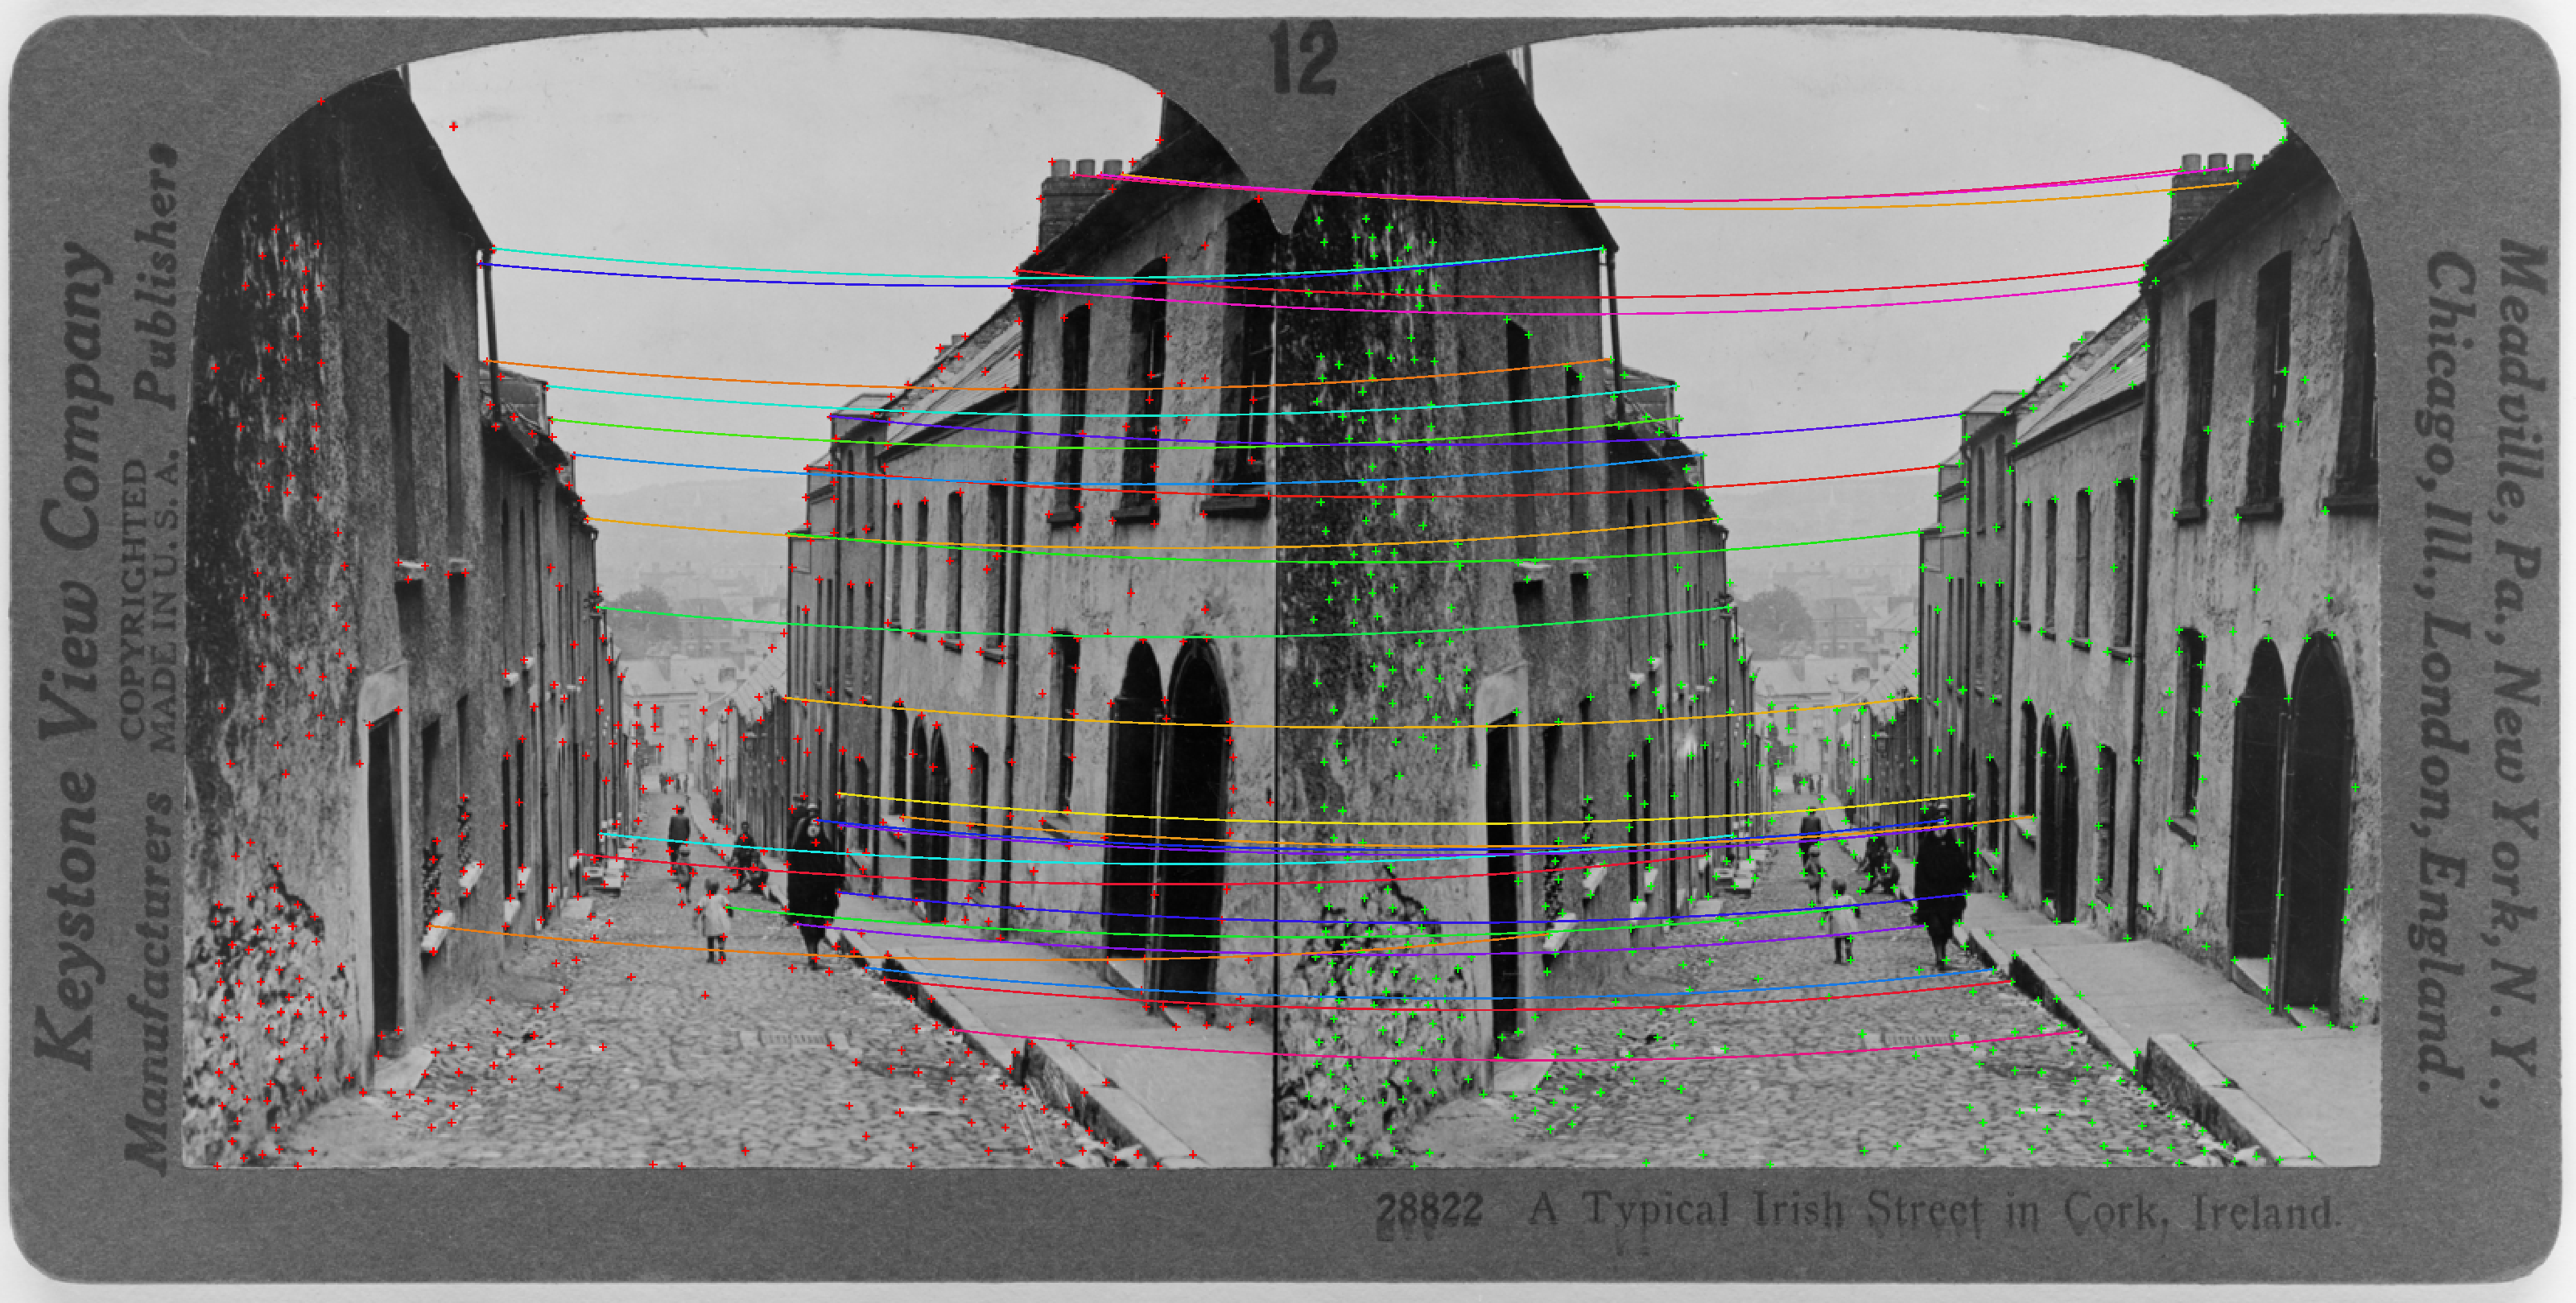
\includegraphics[width=1\linewidth]{images/ass03result1}
	\caption{Result for Image: 3c23727uc.png}
	\label{fig:Result3_1}
\end{figure}

\begin{figure}
	\centering
	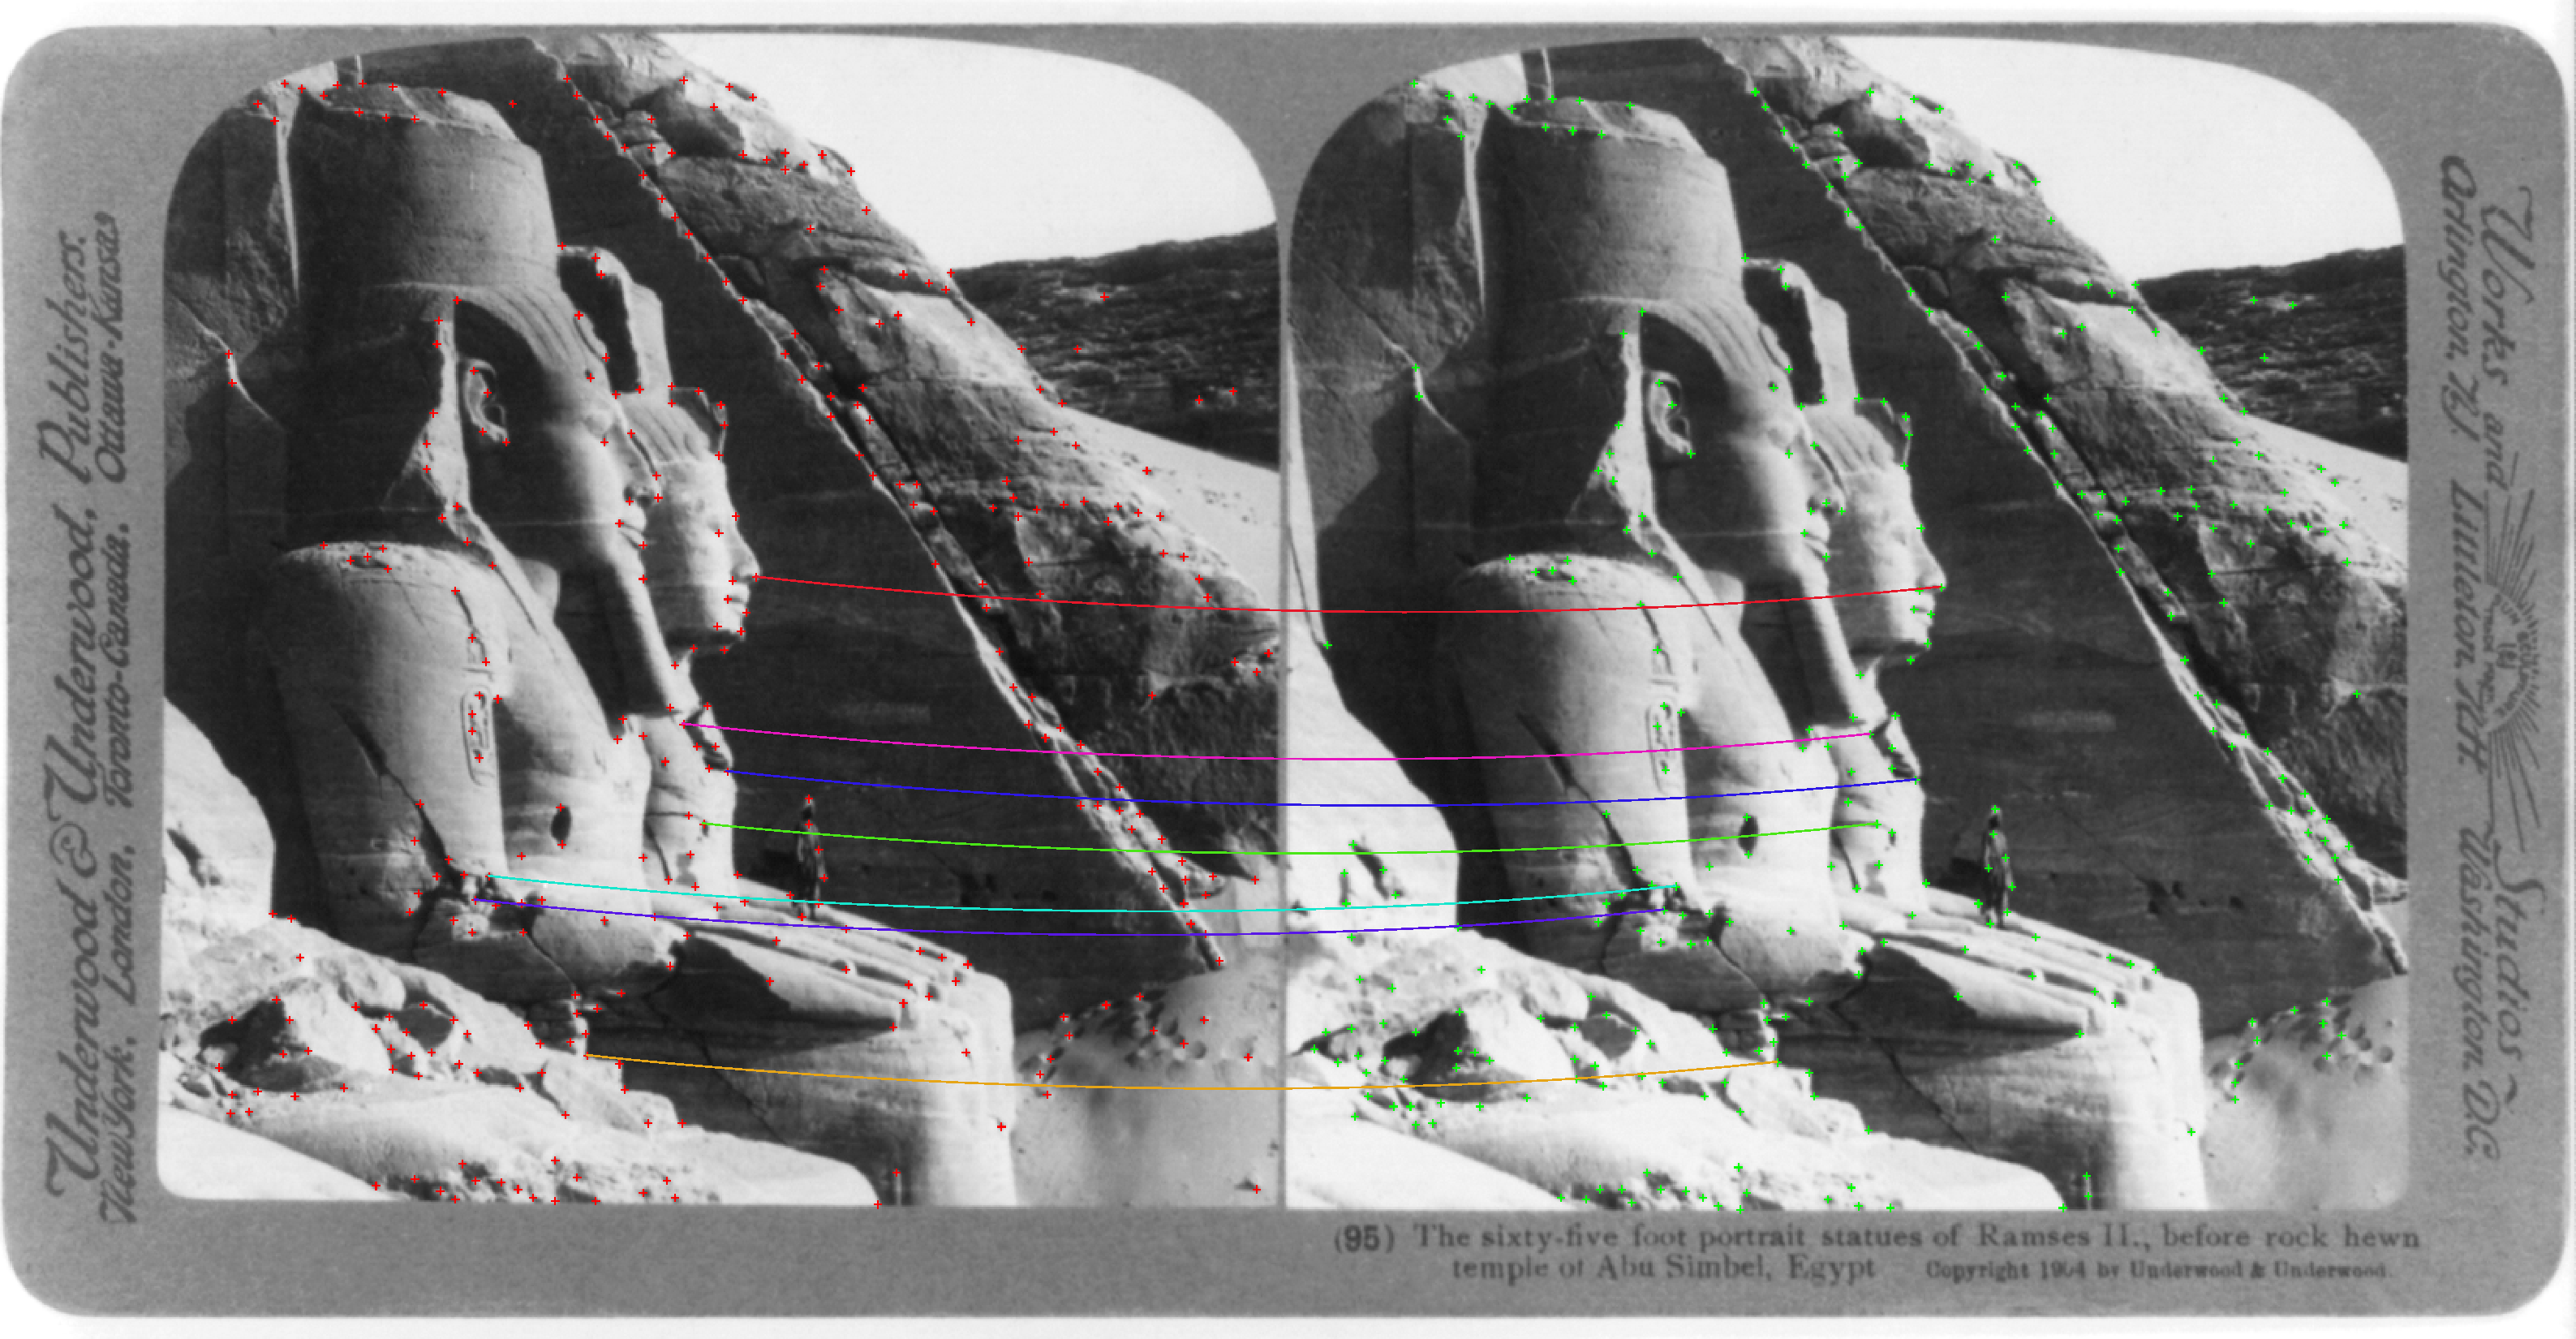
\includegraphics[width=1\linewidth]{images/ass03result2}
	\caption{Result for Image: 3b22263uc.png}
	\label{fig:Result3_2}
\end{figure}

\begin{figure}
	\centering
	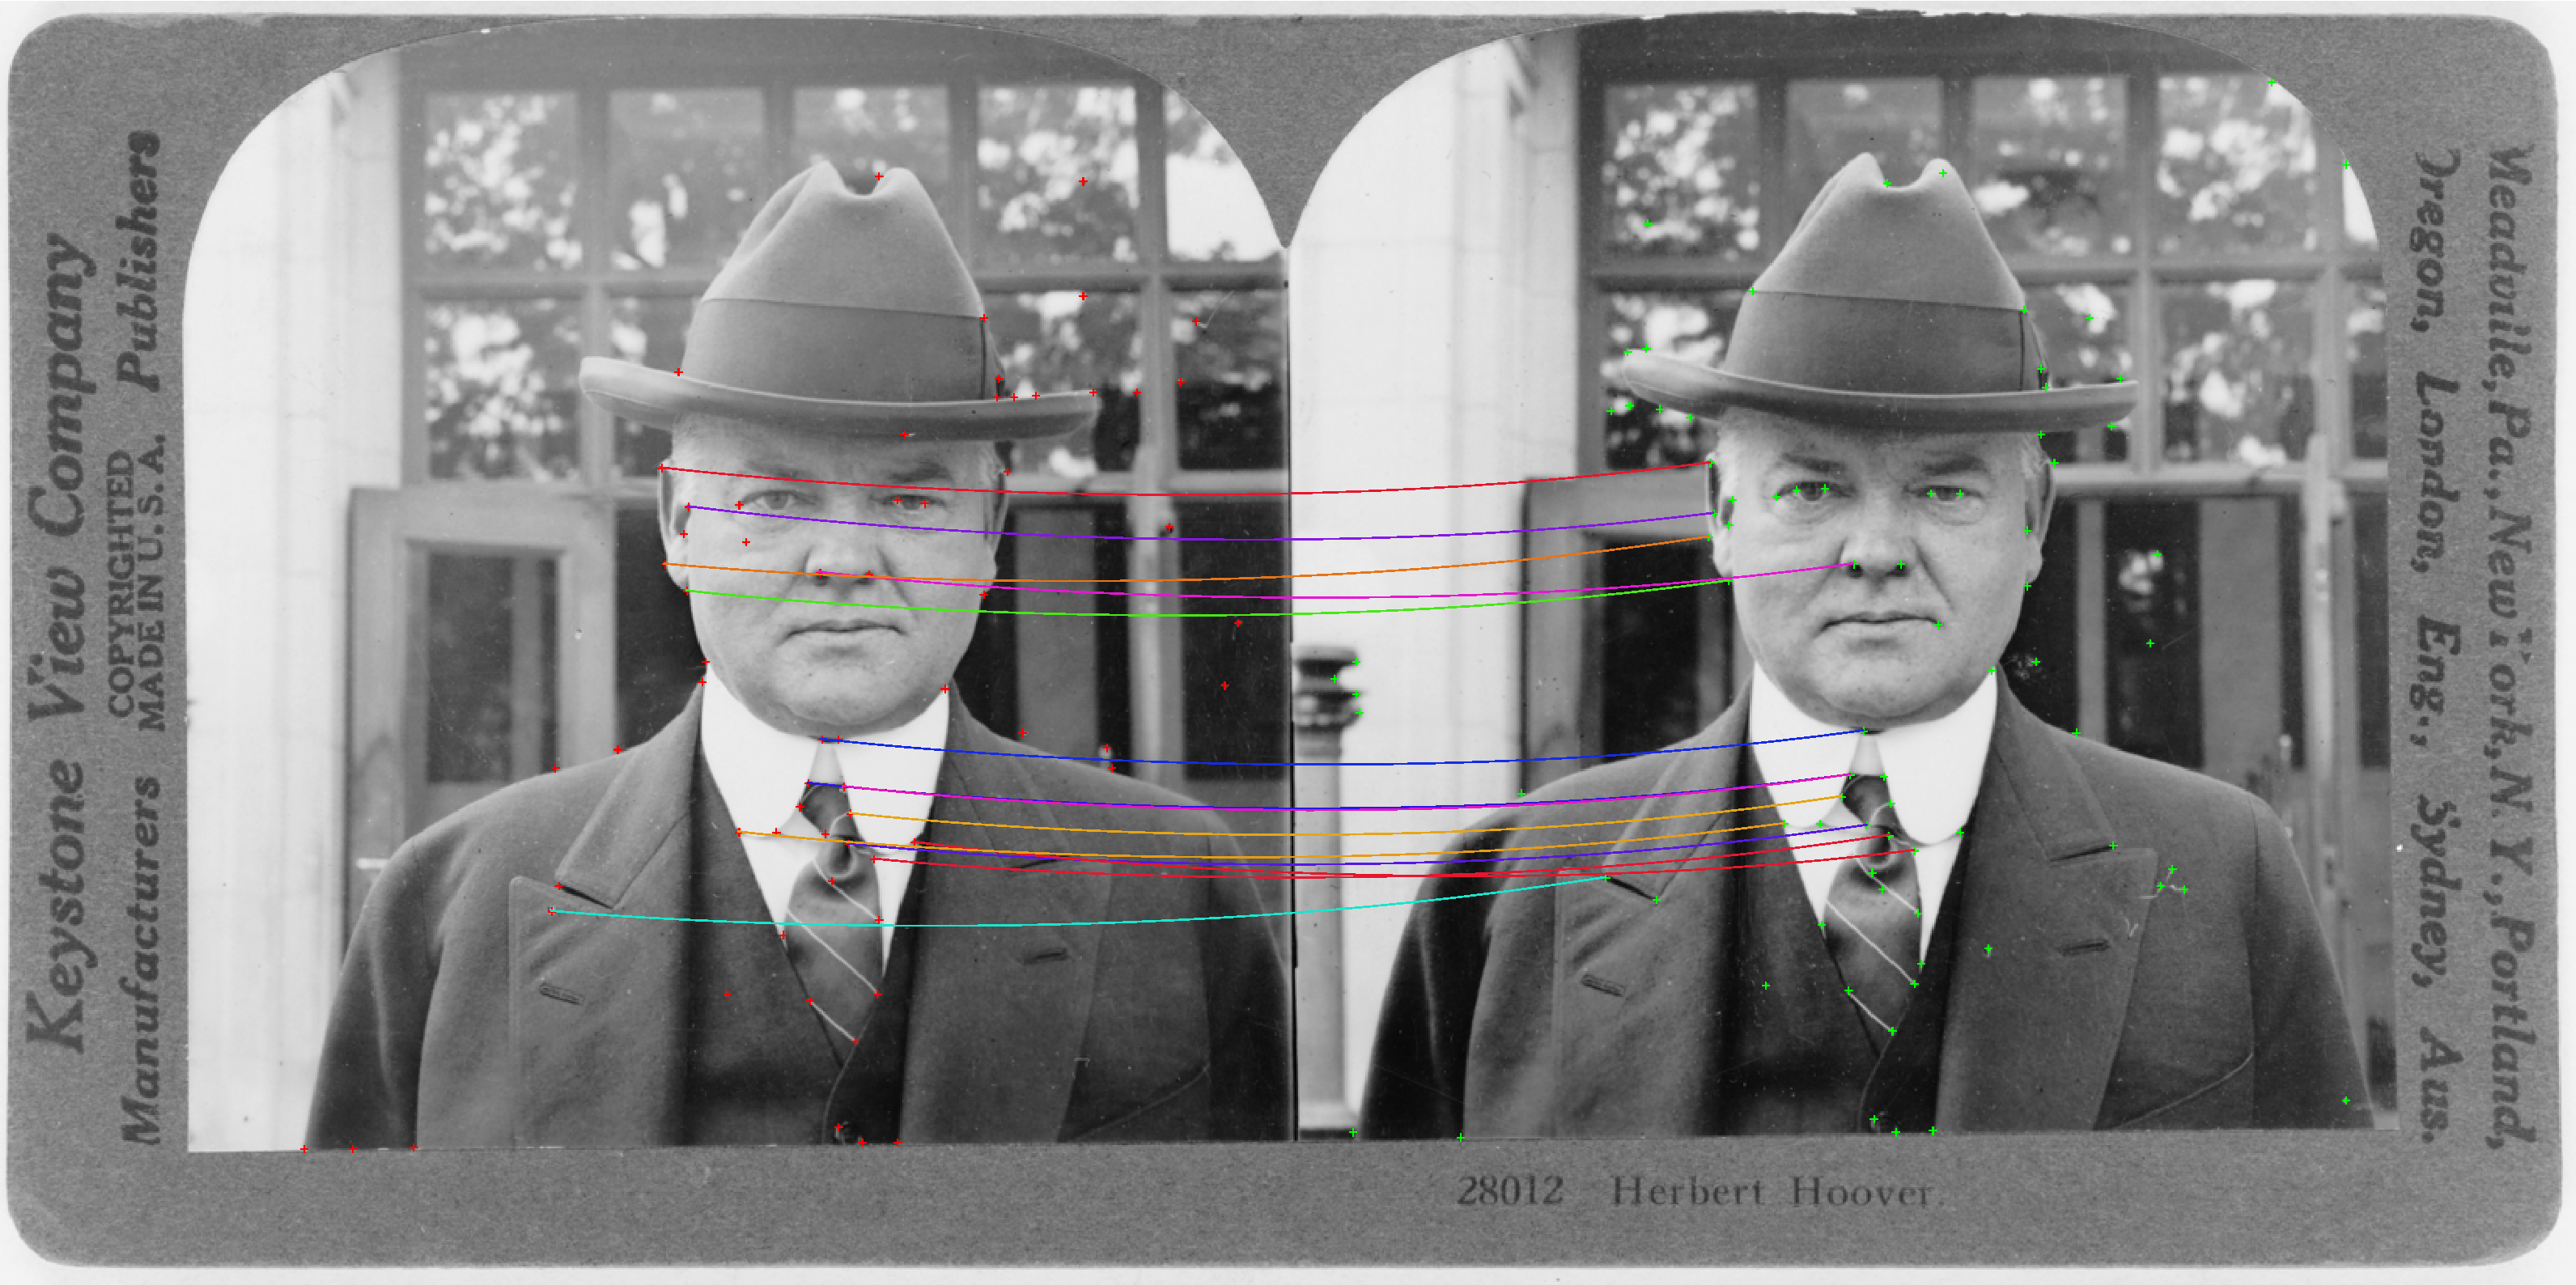
\includegraphics[width=1\linewidth]{images/ass03result3}
	\caption{Result for Image: 3c16514uc.png}
	\label{fig:Result3_3}
\end{figure}

\begin{figure}
	\centering
	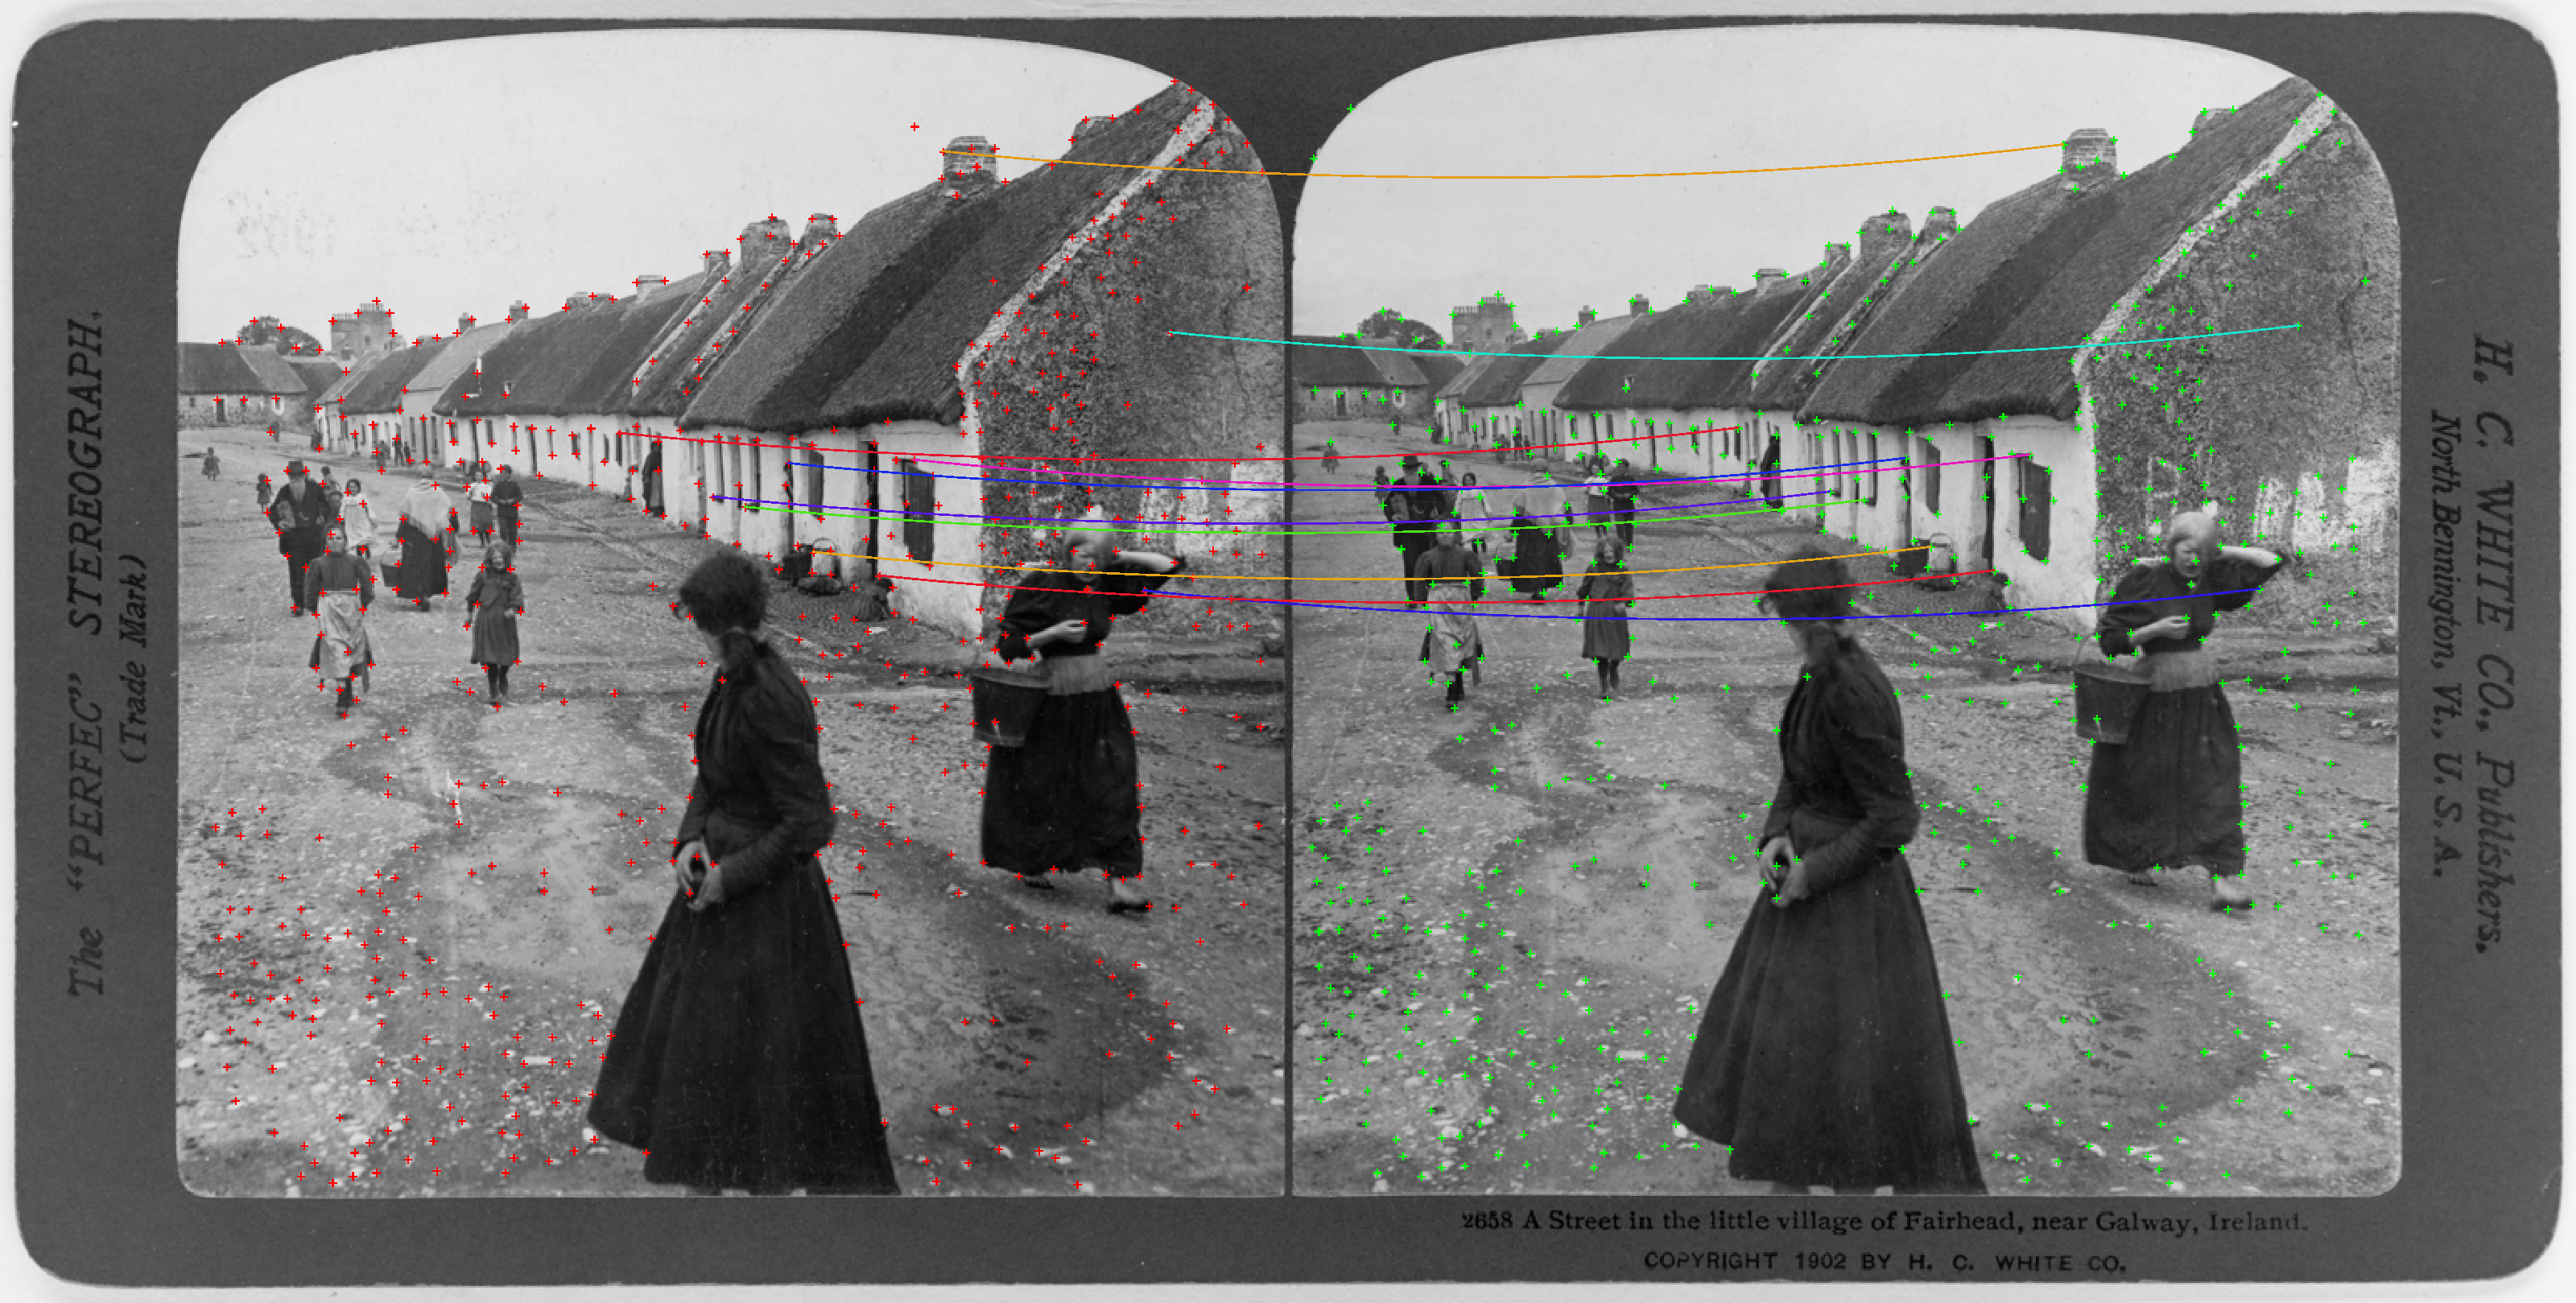
\includegraphics[width=1\linewidth]{images/ass03result4}
	\caption{Result Image: 3c23732uc.png}
	\label{fig:Result3_4}
\end{figure}

\section{Research Question}
\label{section:ResearchQuestion}
\textit{Consider a strategy for coping with outliers inside the ICP algorithm.}

During the step in section \ref{section:Correspondence} where the final correspondence gets established, the error between those point pairs is also calculated and if the error is bigger than a certain threshold (20 was used for these pictures) the pair does not get added to final correspondence list. This way the outliers are not included.







